\section{Results Analysis}

Table~\ref{tab:metrics_summary} reports the test-set results for all model-dataset pairs. Within each dataset, models are sorted by macro F1-score because macro F1 balances precision and recall across classes. The best result for each dataset is highlighted in bold.

\begin{table}[H]
\centering
\caption{Test performance by dataset, sorted by macro F1-score within each dataset.}
\label{tab:metrics_summary}
\resizebox{\linewidth}{!}{%
\begin{tabular}{llrrrr}
\toprule
Dataset & Model & Precision Macro & Recall Macro & F1 Macro & Accuracy \\
\midrule
Yahoo Answers Topics & DistilBERT & \textbf{0.6764} & \textbf{0.6822} & \textbf{0.6750} & \textbf{0.6822} \\
Yahoo Answers Topics & Linear SVM & 0.5740 & 0.5778 & 0.5736 & 0.5778 \\
Yahoo Answers Topics & Naive Bayes & 0.5936 & 0.5500 & 0.5383 & 0.5500 \\
Yahoo Answers Topics & Word2Vec avg & 0.4336 & 0.4433 & 0.4291 & 0.4433 \\
\midrule
AG News Sports vs Business & DistilBERT & \textbf{0.9945} & \textbf{0.9944} & \textbf{0.9944} & \textbf{0.9944} \\
AG News Sports vs Business & Linear SVM & 0.9896 & 0.9895 & 0.9895 & 0.9895 \\
AG News Sports vs Business & Word2Vec avg & 0.9859 & 0.9859 & 0.9859 & 0.9859 \\
AG News Sports vs Business & Naive Bayes & 0.9845 & 0.9843 & 0.9843 & 0.9843 \\
\bottomrule
\end{tabular}
}
\end{table}


\begin{figure}[H]
    \centering
    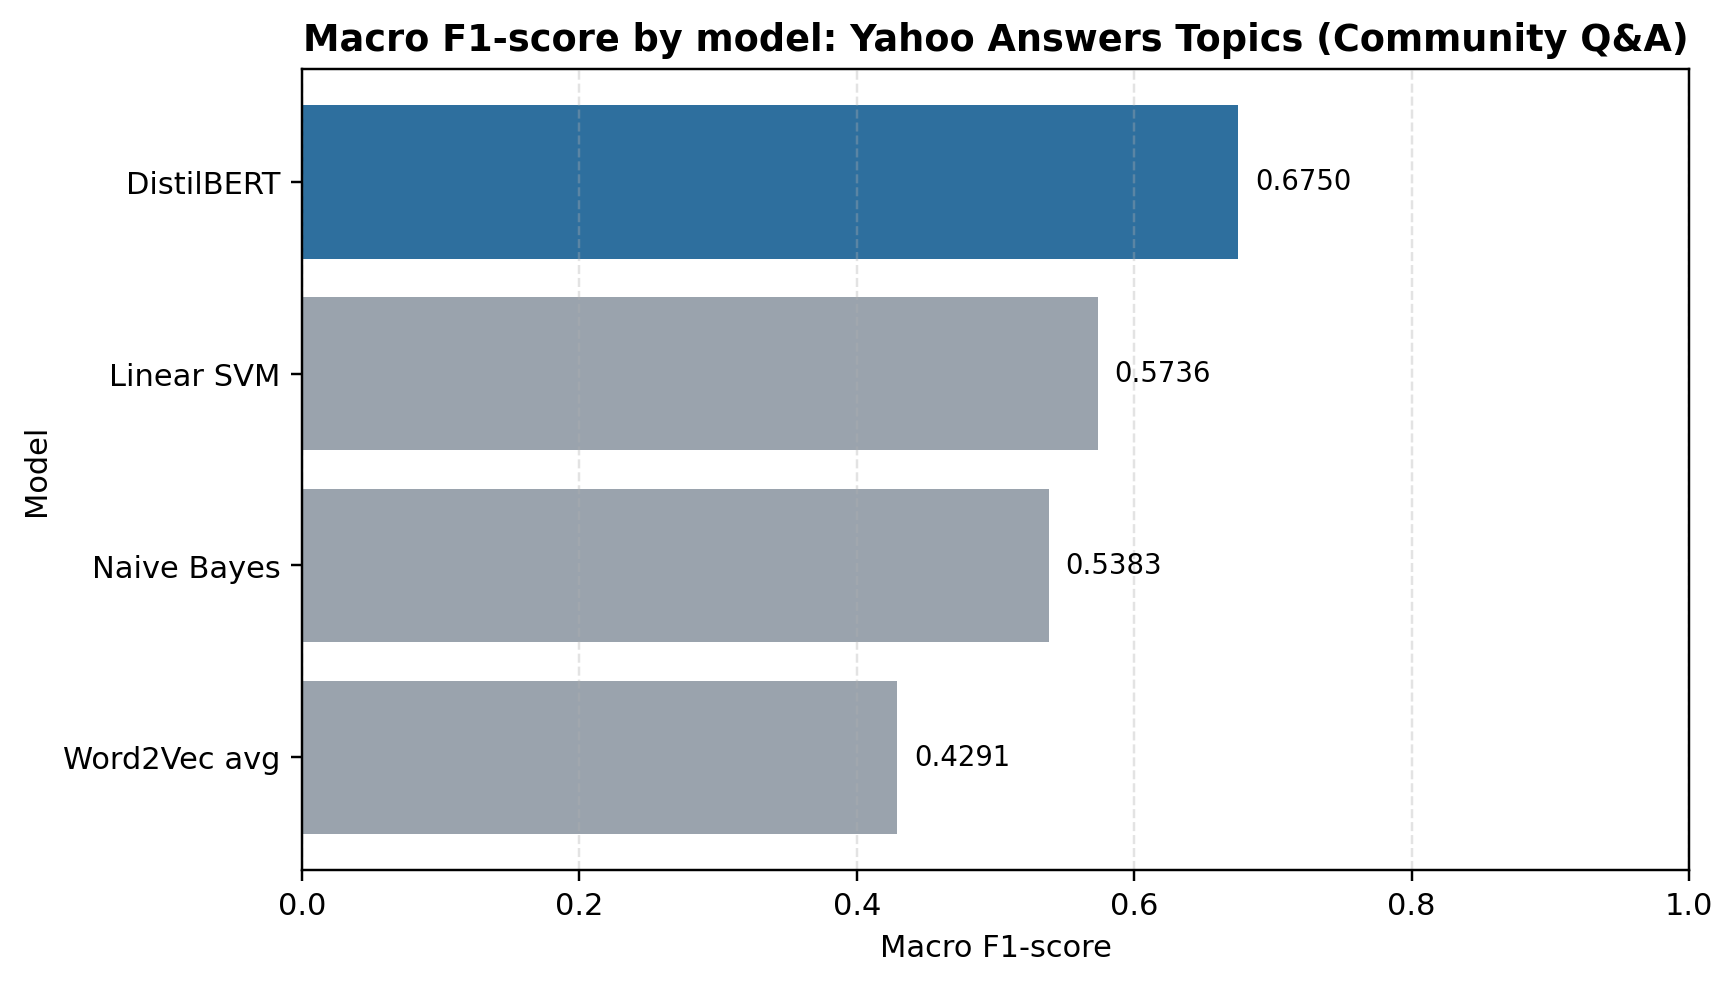
\includegraphics[width=0.86\linewidth]{figures/dataset_1_macro_f1_comparison.png}
    \caption{Macro F1-score comparison on Yahoo Answers Topics.}
    \label{fig:dataset_1_macro_f1}
\end{figure}

\begin{figure}[H]
    \centering
    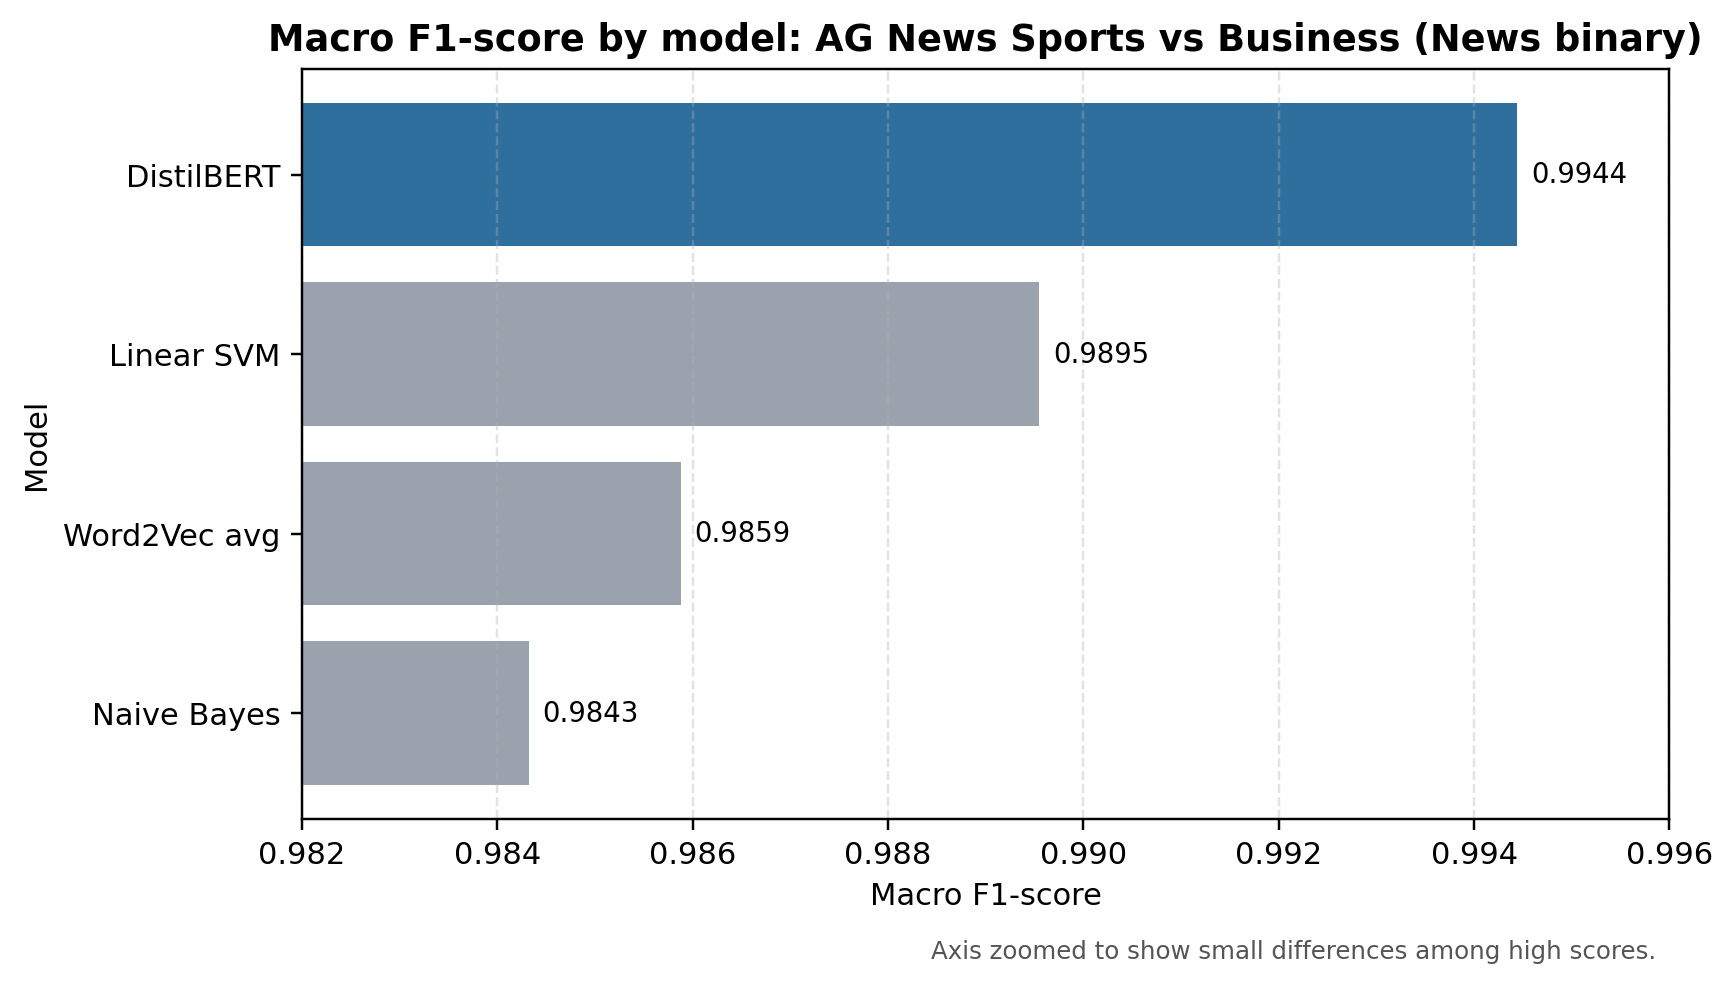
\includegraphics[width=0.86\linewidth]{figures/dataset_2_macro_f1_comparison.png}
    \caption{Macro F1-score comparison on AG News Sports vs Business. The axis is zoomed because all models score above 0.98.}
    \label{fig:dataset_2_macro_f1}
\end{figure}

Yahoo Answers Topics is clearly harder than AG News Sports vs Business. The best macro F1 on Yahoo Answers is 0.6750 from DistilBERT, while the best macro F1 on AG News is 0.9944. The gap is expected because Yahoo Answers has 10 labels, informal community text, and overlapping topic signals. A question may contain terms that are useful for several categories, and short user-generated text can omit context. In contrast, AG News is a binary news classification task where sports and business vocabulary is often more separable.

Precision, recall, and F1 show slightly different aspects of performance. On Yahoo Answers, DistilBERT has the highest macro precision (0.6764), recall (0.6822), and F1-score (0.6750), which means its advantage is not caused by only one metric. SVM has a better macro F1 than Naive Bayes, although Naive Bayes has higher macro precision. This suggests that Naive Bayes is more conservative for some classes, while SVM gives a better precision-recall balance. Word2Vec has the lowest precision, recall, and F1 on Yahoo Answers. Its average pooling representation removes word order and contextual interactions, which is harmful for a noisy multi-class Q\&A dataset.

On AG News, all four models are strong across precision, recall, F1-score, and accuracy. DistilBERT is still the best model, but the margin over SVM is small. SVM, Naive Bayes, and Word2Vec all exceed 0.984 macro F1, showing that clear topic vocabulary can make traditional lexical features highly competitive. These high scores should not be over-generalised to all topic classification tasks. They mainly show that this binary news task is easier and more lexically separable than the Yahoo Answers setting.

Overall, the results support a task-dependent interpretation. Contextual fine-tuning is most useful for the harder multi-class Q\&A dataset. Traditional TF-IDF methods remain strong when the task has clear lexical boundaries. Average Word2Vec document vectors are lightweight, but their loss of order and context makes them less reliable on complex topic structures.
